\chapter{Array e Liste}

\section{Introduzione}

Le strutture dati lineari sono il fondamento dell'organizzazione dei dati in memoria. In questo capitolo studieremo le due strutture lineari fondamentali: gli \textbf{array} e le \textbf{liste concatenate}. Entrambe memorizzano sequenze di elementi, ma con caratteristiche di accesso e modifica molto diverse.

La scelta tra array e liste dipende dalle operazioni che dobbiamo eseguire più frequentemente: accesso casuale, inserimento, cancellazione. Comprendere i trade-off tra queste strutture è essenziale per progettare algoritmi efficienti.

\section{Array}

\subsection{Definizione e proprietà}

\begin{definizione}[Array]
Un \textbf{array} è una struttura dati che memorizza $n$ elementi dello stesso tipo in posizioni di memoria contigue. Ogni elemento è identificato da un \textbf{indice} intero compreso tra $0$ e $n-1$ (o tra $1$ e $n$ a seconda della convenzione).
\end{definizione}

\textbf{Proprietà fondamentali:} Gli array possiedono quattro proprietà distintive. In primo luogo, hanno una \textbf{dimensione fissa}: quando l'array viene creato, la sua dimensione è determinata una volta per tutte e non può essere modificata successivamente. In secondo luogo, consentono \textbf{accesso diretto} a qualsiasi elemento, permettendo di raggiungere l'elemento in posizione $i$ in tempo costante $O(1)$. Una conseguenza della loro implementazione è che gli elementi occupano \textbf{celle consecutive in memoria}, il che consente il calcolo rapido dell'indirizzo di ogni elemento tramite una semplice formula aritmetica. Infine, gli array richiedono \textbf{tipo omogeneo}: tutti gli elementi devono avere lo stesso tipo di dato.

\textbf{Rappresentazione in memoria:}

\begin{center}
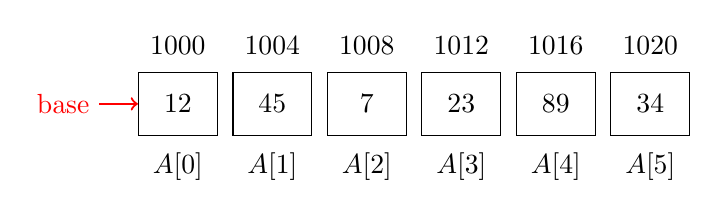
\begin{tikzpicture}[
    array/.style={rectangle, draw, minimum width=1cm, minimum height=0.8cm}
]
    \node[array] (a0) at (0,0) {12};
    \node[array] (a1) at (1.2,0) {45};
    \node[array] (a2) at (2.4,0) {7};
    \node[array] (a3) at (3.6,0) {23};
    \node[array] (a4) at (4.8,0) {89};
    \node[array] (a5) at (6,0) {34};

    \node[below] at (0,-0.5) {$A[0]$};
    \node[below] at (1.2,-0.5) {$A[1]$};
    \node[below] at (2.4,-0.5) {$A[2]$};
    \node[below] at (3.6,-0.5) {$A[3]$};
    \node[below] at (4.8,-0.5) {$A[4]$};
    \node[below] at (6,-0.5) {$A[5]$};

    \node[above] at (0,0.5) {1000};
    \node[above] at (1.2,0.5) {1004};
    \node[above] at (2.4,0.5) {1008};
    \node[above] at (3.6,0.5) {1012};
    \node[above] at (4.8,0.5) {1016};
    \node[above] at (6,0.5) {1020};

    \draw[->, thick, red] (-1,0) -- (a0);
    \node[left, red] at (-1,0) {base};
\end{tikzpicture}

\small \textit{Indirizzi di memoria assumendo 4 byte per elemento}
\end{center}

\subsection{Calcolo dell'indirizzo}

Se $\text{base}$ è l'indirizzo del primo elemento e $\text{size}$ è la dimensione in byte di ogni elemento, l'indirizzo dell'elemento in posizione $i$ è:

\[
\text{address}(A[i]) = \text{base} + i \times \text{size}
\]

Questa formula spiega perché l'accesso è $O(1)$: è una semplice operazione aritmetica.

\subsection{Operazioni su array}

\subsubsection{Accesso}

\begin{lstlisting}[style=pseudocode]
def Accesso(A, i):
    """
    Accede all'elemento in posizione i
    Input: array A, indice i
    Output: A[i]
    Complessità: O(1)
    """
    return A[i]
\end{lstlisting}

\textbf{Complessità temporale:} $\Theta(1)$ \\
\textbf{Complessità spaziale:} $\Theta(1)$

\subsubsection{Modifica}

\begin{lstlisting}[style=pseudocode]
def Modifica(A, i, valore):
    """
    Modifica l'elemento in posizione i
    Complessità: O(1)
    """
    A[i] = valore
\end{lstlisting}

\textbf{Complessità temporale:} $\Theta(1)$ \\
\textbf{Complessità spaziale:} $\Theta(1)$

\subsubsection{Ricerca}

\textbf{Ricerca lineare} (array non ordinato):

\begin{lstlisting}[style=pseudocode]
def RicercaLineare(A, n, chiave):
    """
    Cerca un elemento nell'array
    Input: array A di n elementi, chiave da cercare
    Output: indice se trovato, -1 altrimenti
    """
    for i = 0 to n-1:
        if A[i] == chiave:
            return i
    return -1
\end{lstlisting}

\textbf{Analisi:} La ricerca lineare manifesta comportamenti diversi a seconda della posizione dell'elemento. Nel caso migliore, l'elemento si trova in prima posizione e la ricerca termina con complessità $\Theta(1)$. Nel caso peggiore, che si verifica quando l'elemento non è presente o si trova in ultima posizione, l'algoritmo deve esaminare tutti gli $n$ elementi, richiedendo complessità $\Theta(n)$. Nel caso medio, assumendo che l'elemento sia presente con distribuzione uniforme, il numero atteso di confronti è $\Theta(n)$.

\textbf{Ricerca binaria} (array ordinato):

\begin{lstlisting}[style=pseudocode]
def RicercaBinaria(A, n, chiave):
    """
    Cerca un elemento in un array ordinato
    Input: array ordinato A di n elementi, chiave
    Output: indice se trovato, -1 altrimenti
    Complessità: O(log n)
    """
    sinistra = 0
    destra = n - 1

    while sinistra <= destra:
        medio = (sinistra + destra) // 2

        if A[medio] == chiave:
            return medio
        elif A[medio] < chiave:
            sinistra = medio + 1
        else:
            destra = medio - 1

    return -1
\end{lstlisting}

\textbf{Analisi della ricerca binaria:}

Sia $T(n)$ il numero di confronti nel caso peggiore. Ad ogni iterazione, la dimensione dell'intervallo di ricerca si dimezza:

\[
T(n) = T(n/2) + O(1)
\]

Per il Master Theorem (caso 2 con $a=1, b=2, f(n)=O(1)$):
\[
T(n) = \Theta(\log n)
\]

\begin{teorema}[Correttezza della ricerca binaria]
Se l'array $A$ è ordinato, l'algoritmo di ricerca binaria termina e restituisce l'indice della chiave se presente, $-1$ altrimenti.
\end{teorema}

\begin{proof}
Dimostrazione per invariante di ciclo. L'invariante è: "Se la chiave è presente nell'array, allora si trova nell'intervallo $[sinistra, destra]$".

\textbf{Inizializzazione:} Prima del primo ciclo, $sinistra = 0$ e $destra = n-1$, quindi l'intervallo copre tutto l'array. ✓

\textbf{Mantenimento:} Ad ogni iterazione:
\begin{itemize}
    \item Se $A[medio] = chiave$, l'algoritmo termina correttamente.
    \item Se $A[medio] < chiave$, per l'ordinamento, la chiave può essere solo a destra di $medio$, quindi restringiamo a $[medio+1, destra]$. ✓
    \item Se $A[medio] > chiave$, per l'ordinamento, la chiave può essere solo a sinistra di $medio$, quindi restringiamo a $[sinistra, medio-1]$. ✓
\end{itemize}

\textbf{Terminazione:} Il ciclo termina quando $sinistra > destra$ (intervallo vuoto) o quando troviamo la chiave. Se l'intervallo diventa vuoto, la chiave non è presente. ✓
\end{proof}

\subsubsection{Inserimento}

\textbf{Inserimento in coda} (se c'è spazio):

\begin{lstlisting}[style=pseudocode]
def InserimentoCoda(A, n, valore):
    """
    Inserisce un elemento in coda
    Precondizione: n < capacità dell'array
    Complessità: O(1)
    """
    A[n] = valore
    return n + 1  // nuova dimensione
\end{lstlisting}

\textbf{Complessità:} $\Theta(1)$

\textbf{Inserimento in posizione arbitraria:}

\begin{lstlisting}[style=pseudocode]
def Inserimento(A, n, i, valore):
    """
    Inserisce valore in posizione i
    Richiede lo shift degli elementi successivi
    Complessità: O(n)
    """
    // Shift elementi verso destra
    for j = n-1 down to i:
        A[j+1] = A[j]

    A[i] = valore
    return n + 1
\end{lstlisting}

\textbf{Analisi:} L'inserimento in una posizione arbitraria presenta complessità variabili. Nel caso migliore, l'inserimento avviene in coda (dove non è necessario alcuno shift), con complessità $\Theta(1)$. Nel caso peggiore, inserire un elemento in testa richiede di spostare tutti gli $n$ elementi esistenti verso destra, risultando in complessità $\Theta(n)$. Nel caso medio, assumendo distribuzione uniforme della posizione di inserimento, il numero atteso di shift è $n/2$, mantenendo complessità $\Theta(n)$.

\begin{center}
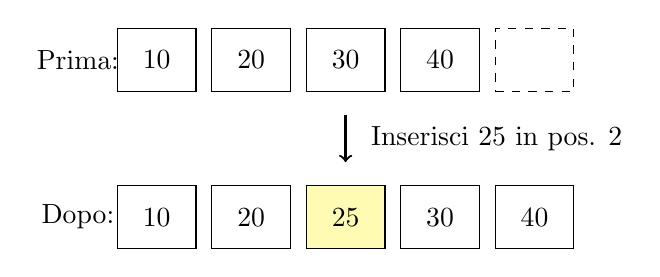
\begin{tikzpicture}[
    array/.style={rectangle, draw, minimum width=1cm, minimum height=0.8cm}
]
    % Array prima
    \node at (-1, 1.5) {Prima:};
    \node[array] (a0) at (0,1.5) {10};
    \node[array] (a1) at (1.2,1.5) {20};
    \node[array] (a2) at (2.4,1.5) {30};
    \node[array] (a3) at (3.6,1.5) {40};
    \node[array, dashed] (a4) at (4.8,1.5) {};

    % Freccia
    \draw[->, thick] (2.4, 0.8) -- (2.4, 0.2);
    \node[right] at (2.6, 0.5) {Inserisci 25 in pos. 2};

    % Array dopo
    \node at (-1, -0.5) {Dopo:};
    \node[array] (b0) at (0,-0.5) {10};
    \node[array] (b1) at (1.2,-0.5) {20};
    \node[array, fill=yellow!30] (b2) at (2.4,-0.5) {25};
    \node[array] (b3) at (3.6,-0.5) {30};
    \node[array] (b4) at (4.8,-0.5) {40};
\end{tikzpicture}
\end{center}

\subsubsection{Cancellazione}

\begin{lstlisting}[style=pseudocode]
def Cancellazione(A, n, i):
    """
    Cancella l'elemento in posizione i
    Richiede lo shift degli elementi successivi
    Complessità: O(n)
    """
    // Shift elementi verso sinistra
    for j = i to n-2:
        A[j] = A[j+1]

    return n - 1  // nuova dimensione
\end{lstlisting}

\textbf{Analisi:} L'analisi della cancellazione rispecchia quella dell'inserimento, poiché entrambe le operazioni richiedono shift di elementi. Nel caso migliore, cancellare l'ultimo elemento non richiede alcuno shift, con complessità $\Theta(1)$. Nel caso peggiore, cancellare il primo elemento costringe a spostare tutti i rimanenti $n-1$ elementi verso sinistra, risultando in complessità $\Theta(n)$. Nel caso medio, la complessità rimane $\Theta(n)$.

\subsection{Array dinamici}

Gli array statici hanno dimensione fissa, il che è limitante. Gli \textbf{array dinamici} (dynamic arrays, in C++ \texttt{std::vector}, in Java \texttt{ArrayList}, in Python \texttt{list}) risolvono questo problema.

\textbf{Strategia di raddoppio:} Quando l'array raggiunge la sua capacità massima e deve accogliere un nuovo elemento, si alloca un nuovo array di dimensione doppia rispetto al precedente. Successivamente, tutti gli elementi dell'array originale vengono copiati nel nuovo array, e il vecchio array viene deallocato. Questo meccanismo, sebbene possa sembrare costoso per singoli inserimenti (che occasionalmente richiedono $O(n)$), risulta straordinariamente efficiente in analisi ammortizzata, come dimostreremo.

\begin{lstlisting}[style=pseudocode]
def InserimentoDinamico(A, n, capacità, valore):
    """
    Inserisce in un array dinamico
    """
    if n == capacità:
        // Array pieno, raddoppia
        nuova_capacità = 2 * capacità
        B = nuovo array di dimensione nuova_capacità

        for i = 0 to n-1:
            B[i] = A[i]

        A = B
        capacità = nuova_capacità

    A[n] = valore
    return n + 1, capacità
\end{lstlisting}

\textbf{Analisi ammortizzata:}

Un singolo inserimento può costare $\Theta(n)$ se richiede raddoppio, ma non tutti gli inserimenti richiedono raddoppio.

\begin{teorema}[Costo ammortizzato dell'inserimento in array dinamico]
Il costo ammortizzato di un inserimento in un array dinamico con strategia di raddoppio è $\Theta(1)$.
\end{teorema}

\begin{proof}
Consideriamo una sequenza di $n$ inserimenti partendo da un array vuoto.

Gli inserimenti che richiedono raddoppio avvengono quando $n = 1, 2, 4, 8, 16, \ldots, 2^k$ dove $2^k \leq n < 2^{k+1}$.

Il costo totale è:
\begin{align*}
C(n) &= n + \sum_{i=0}^{\lfloor \log n \rfloor} 2^i \\
     &= n + (2^{\lfloor \log n \rfloor + 1} - 1) \\
     &< n + 2n = 3n
\end{align*}

Il costo ammortizzato per operazione è:
\[
\frac{C(n)}{n} < \frac{3n}{n} = 3 = O(1)
\]
\end{proof}

\subsection{Tabella riassuntiva delle complessità}

\begin{center}
\begin{tabular}{|l|c|c|c|}
\hline
\textbf{Operazione} & \textbf{Array statico} & \textbf{Array dinamico} \\
\hline
Accesso & $O(1)$ & $O(1)$ \\
Modifica & $O(1)$ & $O(1)$ \\
Ricerca (non ordinato) & $O(n)$ & $O(n)$ \\
Ricerca (ordinato) & $O(\log n)$ & $O(\log n)$ \\
Inserimento in coda & $O(1)^*$ & $O(1)$ ammortizzato \\
Inserimento in posizione $i$ & $O(n)$ & $O(n)$ \\
Cancellazione & $O(n)$ & $O(n)$ \\
\hline
\multicolumn{3}{l}{\small $^*$ se c'è spazio disponibile} \\
\end{tabular}
\end{center}

\section{Liste concatenate}

\subsection{Definizione e struttura}

\begin{definizione}[Lista concatenata semplice]
Una \textbf{lista concatenata semplice} è una sequenza di nodi, dove ogni nodo contiene due elementi essenziali: un \textbf{dato} (il valore memorizzato) e un \textbf{puntatore} al nodo successivo nella sequenza. Il primo nodo della lista è speciale e viene chiamato \textbf{testa} (head), mentre l'ultimo nodo ha il suo puntatore impostato a \texttt{NULL} per indicare la fine della lista.
\end{definizione}

\textbf{Struttura del nodo:}

\begin{lstlisting}[style=pseudocode]
class Nodo:
    def __init__(self, dato):
        self.dato = dato
        self.next = None
\end{lstlisting}

\textbf{Rappresentazione grafica:}

\begin{center}
\begin{tikzpicture}[
    node/.style={rectangle split, rectangle split parts=2, draw, rectangle split horizontal},
    >=stealth
]
    \node[node] (n1) at (0,0) {12 \nodepart{two} };
    \node[node] (n2) at (2.5,0) {45 \nodepart{two} };
    \node[node] (n3) at (5,0) {7 \nodepart{two} };
    \node[node] (n4) at (7.5,0) {23 \nodepart{two} };

    \draw[->] (n1.two east) -- (n2);
    \draw[->] (n2.two east) -- (n3);
    \draw[->] (n3.two east) -- (n4);
    \draw[->] (n4.two east) -- ++(1,0) node[right] {NULL};

    \draw[->] (-1.5,0) -- (n1) node[midway, above] {head};
\end{tikzpicture}
\end{center}

\subsection{Operazioni su liste concatenate}

\subsubsection{Inserimento in testa}

\begin{lstlisting}[style=pseudocode]
def InserimentoTesta(head, valore):
    """
    Inserisce un nuovo nodo in testa alla lista
    Input: testa della lista, valore da inserire
    Output: nuova testa
    Complessità: O(1)
    """
    nuovo = Nodo(valore)
    nuovo.next = head
    return nuovo
\end{lstlisting}

\textbf{Complessità:} $\Theta(1)$ \\
\textbf{Visualizzazione:}

\begin{center}
\begin{tikzpicture}[
    node/.style={rectangle split, rectangle split parts=2, draw, rectangle split horizontal},
    >=stealth
]
    % Stato finale
    \node[node, fill=yellow!30] (new) at (0,0) {99 \nodepart{two} };
    \node[node] (n1) at (2.5,0) {12 \nodepart{two} };
    \node[node] (n2) at (5,0) {45 \nodepart{two} };

    \draw[->] (new.two east) -- (n1);
    \draw[->] (n1.two east) -- (n2);
    \draw[->] (n2.two east) -- ++(1,0) node[right] {NULL};

    \draw[->] (-1.5,0) -- (new) node[midway, above] {head};
\end{tikzpicture}
\end{center}

\subsubsection{Inserimento in coda}

\begin{lstlisting}[style=pseudocode]
def InserimentoCoda(head, valore):
    """
    Inserisce un nuovo nodo in coda alla lista
    Complessità: O(n)
    """
    nuovo = Nodo(valore)

    if head == None:
        return nuovo

    corrente = head
    while corrente.next != None:
        corrente = corrente.next

    corrente.next = nuovo
    return head
\end{lstlisting}

\textbf{Complessità:} $\Theta(n)$ (dobbiamo scorrere tutta la lista)

\textbf{Ottimizzazione:} Mantenere un puntatore alla coda riduce la complessità a $\Theta(1)$.

\subsubsection{Inserimento in posizione}

\begin{lstlisting}[style=pseudocode]
def InserimentoPosizione(head, valore, posizione):
    """
    Inserisce un nodo nella posizione specificata (0-based)
    Complessità: O(n)
    """
    if posizione == 0:
        return InserimentoTesta(head, valore)

    nuovo = Nodo(valore)
    corrente = head

    for i = 0 to posizione-2:
        if corrente == None:
            return head  // posizione non valida
        corrente = corrente.next

    if corrente != None:
        nuovo.next = corrente.next
        corrente.next = nuovo

    return head
\end{lstlisting}

\textbf{Complessità:} $O(n)$

\subsubsection{Cancellazione in testa}

\begin{lstlisting}[style=pseudocode]
def CancellazioneTesta(head):
    """
    Cancella il primo nodo
    Complessità: O(1)
    """
    if head == None:
        return None

    nuova_head = head.next
    // In linguaggi con garbage collection, head viene deallocato automaticamente
    return nuova_head
\end{lstlisting}

\textbf{Complessità:} $\Theta(1)$

\subsubsection{Cancellazione di un valore}

\begin{lstlisting}[style=pseudocode]
def CancellaValore(head, valore):
    """
    Cancella il primo nodo con il valore specificato
    Complessità: O(n)
    """
    if head == None:
        return None

    // Caso speciale: testa da cancellare
    if head.dato == valore:
        return head.next

    corrente = head
    while corrente.next != None:
        if corrente.next.dato == valore:
            corrente.next = corrente.next.next
            return head
        corrente = corrente.next

    return head  // valore non trovato
\end{lstlisting}

\textbf{Complessità:} $O(n)$

\subsubsection{Ricerca}

\begin{lstlisting}[style=pseudocode]
def Ricerca(head, valore):
    """
    Cerca un valore nella lista
    Output: il nodo se trovato, None altrimenti
    Complessità: O(n)
    """
    corrente = head
    while corrente != None:
        if corrente.dato == valore:
            return corrente
        corrente = corrente.next
    return None
\end{lstlisting}

\textbf{Complessità:} $O(n)$ in tutti i casi

\subsubsection{Attraversamento}

\begin{lstlisting}[style=pseudocode]
def Stampa(head):
    """
    Stampa tutti gli elementi della lista
    Complessità: O(n)
    """
    corrente = head
    while corrente != None:
        print(corrente.dato)
        corrente = corrente.next
\end{lstlisting}

\textbf{Complessità:} $\Theta(n)$

\subsection{Liste concatenate doppie}

\begin{definizione}[Lista concatenata doppia]
Una \textbf{lista concatenata doppia} è una sequenza di nodi dove ogni nodo contiene:
\begin{itemize}
    \item Un dato
    \item Un puntatore al nodo \textbf{successivo} (\texttt{next})
    \item Un puntatore al nodo \textbf{precedente} (\texttt{prev})
\end{itemize}
\end{definizione}

\textbf{Struttura del nodo:}

\begin{lstlisting}[style=pseudocode]
class NodoDoppio:
    def __init__(self, dato):
        self.dato = dato
        self.next = None
        self.prev = None
\end{lstlisting}

\textbf{Rappresentazione grafica:}

\begin{center}
\begin{tikzpicture}[
    node/.style={rectangle split, rectangle split parts=3, draw, rectangle split horizontal},
    >=stealth
]
    \node[node] (n1) at (0,0) { \nodepart{two} 12 \nodepart{three} };
    \node[node] (n2) at (3,0) { \nodepart{two} 45 \nodepart{three} };
    \node[node] (n3) at (6,0) { \nodepart{two} 7 \nodepart{three} };

    \draw[->] (n1.three east) -- (n2) node[midway, above] {\tiny next};
    \draw[->] (n2) -- (n1.three east) node[midway, below] {\tiny prev};

    \draw[->] (n2.three east) -- (n3) node[midway, above] {\tiny next};
    \draw[->] (n3) -- (n2.three east) node[midway, below] {\tiny prev};

    \draw[->] (-1,0) -- (n1);
    \draw[->] (n3.three east) -- ++(1,0) node[right] {NULL};
    \draw[->] (n1.one west) -- ++(-0.5,0) node[left] {NULL};
\end{tikzpicture}
\end{center}

\textbf{Vantaggi e svantaggi:} Le liste doppie offrono tre vantaggi significativi rispetto alle liste semplici. Primo, consentono lo \textbf{scorrimento bidirezionale}: è possibile muoversi avanti e indietro nella lista con uguale facilità. Secondo, permettono la \textbf{cancellazione di un nodo} in tempo $O(1)$ se disponiamo già di un puntatore al nodo da cancellare, poiché possiamo accedere direttamente ai nodi precedente e successivo. Terzo, agevolano l'\textbf{inserimento prima di un nodo} in tempo costante. D'altro canto, le liste doppie richiedono \textbf{maggiore uso di memoria} a causa del puntatore aggiuntivo per ogni nodo, e comportano \textbf{maggiore complessità nel mantenere gli invarianti} dei puntatori durante le operazioni di modifica.

\subsubsection{Cancellazione dato il nodo (lista doppia)}

\begin{lstlisting}[style=pseudocode]
def CancellaNodo(nodo):
    """
    Cancella un nodo data la sua posizione
    SOLO per liste doppie
    Complessità: O(1)
    """
    if nodo.prev != None:
        nodo.prev.next = nodo.next

    if nodo.next != None:
        nodo.next.prev = nodo.prev

    // nodo viene deallocato
\end{lstlisting}

\textbf{Complessità:} $\Theta(1)$ --- questo è un grande vantaggio rispetto alla lista semplice!

\subsection{Liste circolari}

\begin{definizione}[Lista circolare]
Una \textbf{lista circolare} è una lista concatenata in cui l'ultimo nodo punta al primo (invece di \texttt{NULL}).
\end{definizione}

\begin{center}
\begin{tikzpicture}[
    node/.style={rectangle split, rectangle split parts=2, draw, rectangle split horizontal},
    >=stealth
]
    \node[node] (n1) at (0,0) {12 \nodepart{two} };
    \node[node] (n2) at (2,0) {45 \nodepart{two} };
    \node[node] (n3) at (4,0) {7 \nodepart{two} };
    \node[node] (n4) at (6,0) {23 \nodepart{two} };

    \draw[->] (n1.two east) -- (n2);
    \draw[->] (n2.two east) -- (n3);
    \draw[->] (n3.two east) -- (n4);
    \draw[->, red, thick] (n4.two east) to[out=30, in=-30] (n1);

    \draw[->] (-1,0) -- (n1) node[midway, above] {head};
\end{tikzpicture}
\end{center}

\textbf{Applicazioni:} Round-robin scheduling, buffer circolari.

\subsection{Confronto array vs liste}

\begin{center}
\begin{tabular}{|l|c|c|}
\hline
\textbf{Operazione} & \textbf{Array} & \textbf{Lista concatenata} \\
\hline
Accesso al k-esimo elemento & $O(1)$ & $O(k)$ \\
Ricerca elemento & $O(n)$ & $O(n)$ \\
Inserimento in testa & $O(n)$ & $O(1)$ \\
Inserimento in coda & $O(1)^*$ & $O(n)$ o $O(1)^{**}$ \\
Inserimento in mezzo & $O(n)$ & $O(n)$ \\
Cancellazione in testa & $O(n)$ & $O(1)$ \\
Cancellazione in coda & $O(1)$ & $O(n)$ o $O(1)^{**}$ \\
Uso memoria & Compatto & Extra per puntatori \\
Località di cache & Ottima & Scarsa \\
Dimensione & Fissa o dinamica & Dinamica \\
\hline
\multicolumn{3}{l}{\small $^*$ se c'è spazio; $^{**}$ se si mantiene puntatore alla coda} \\
\end{tabular}
\end{center}

\section{Applicazioni pratiche}

\subsection{Implementazione di buffer}

Gli array circolari sono usati per implementare buffer FIFO efficienti in sistemi embedded e streaming.

\subsection{Undo/Redo in editor}

Le liste doppie permettono di navigare avanti e indietro nella storia delle modifiche.

\subsection{Rappresentazione di polinomi}

Un polinomio sparso $P(x) = 3x^{100} + 5x^{50} + 2$ può essere rappresentato efficientemente con una lista di coppie (coefficiente, esponente).

\subsection{Gestione memoria dinamica}

I sistemi operativi usano liste concatenate per gestire blocchi di memoria liberi (free lists).

\section{Algoritmi avanzati su liste}

\subsection{Inversione di una lista}

\begin{lstlisting}[style=pseudocode]
def Inverti(head):
    """
    Inverte una lista concatenata
    Complessità: O(n) tempo, O(1) spazio
    """
    prev = None
    corrente = head

    while corrente != None:
        prossimo = corrente.next
        corrente.next = prev
        prev = corrente
        corrente = prossimo

    return prev
\end{lstlisting}

\textbf{Complessità:} $\Theta(n)$ tempo, $\Theta(1)$ spazio

\subsection{Rilevazione di cicli (Floyd's Algorithm)}

\begin{lstlisting}[style=pseudocode]
def HaCiclo(head):
    """
    Rileva se una lista ha un ciclo
    Algoritmo della tartaruga e della lepre
    Complessità: O(n) tempo, O(1) spazio
    """
    if head == None:
        return False

    lento = head
    veloce = head

    while veloce != None and veloce.next != None:
        lento = lento.next
        veloce = veloce.next.next

        if lento == veloce:
            return True

    return False
\end{lstlisting}

\begin{teorema}[Correttezza dell'algoritmo di Floyd]
Se una lista ha un ciclo, i puntatori lento e veloce si incontreranno.
\end{teorema}

\begin{proof}[Idea]
Quando il puntatore lento entra nel ciclo, il veloce è già nel ciclo. La distanza tra loro diminuisce di 1 ad ogni iterazione (il veloce avanza di 2, il lento di 1). Eventualmente la distanza diventa 0.
\end{proof}

\subsection{Trovare il punto medio}

\begin{lstlisting}[style=pseudocode]
def TrovaMedio(head):
    """
    Trova il nodo medio della lista
    Complessità: O(n) tempo, O(1) spazio
    """
    if head == None:
        return None

    lento = head
    veloce = head

    while veloce.next != None and veloce.next.next != None:
        lento = lento.next
        veloce = veloce.next.next

    return lento
\end{lstlisting}

\section{Conclusioni}

Array e liste concatenate sono le strutture dati lineari fondamentali. La scelta tra le due dipende dalle operazioni predominanti:

\begin{itemize}
    \item \textbf{Usa array} quando: accesso casuale frequente, dimensione nota, località di cache importante
    \item \textbf{Usa liste} quando: inserimenti/cancellazioni frequenti, dimensione variabile, no accesso casuale
\end{itemize}

Molte strutture dati complesse (stack, code, hash table con chaining) sono costruite su questi fondamenti.

\textbf{Punti chiave:} Le caratteristiche distintive delle strutture lineari esaminate meritano una revisione. Gli array eccellono nell'accesso rapido ($O(1)$) ma penalizzano inserimenti e cancellazioni ($O(n)$). Le liste concatenate invertono questo compromesso, permettendo operazioni di inserimento e cancellazione in testa in tempo $O(1)$, ma richiedendo accesso sequenziale ($O(n)$) a elementi arbitrari. Le liste doppie aggiungono la proprietà speciale di permettere la cancellazione di un nodo in $O(1)$ se conosciamo già il nodo. Infine, gli array dinamici offrono il meglio di due mondi: accesso rapido come gli array statici e inserimenti ammortizzati in $O(1)$ grazie alla strategia di raddoppio.
